\section{Implementation}\label{sec:impl}


We implemented the formal transformation rule for the distributed training
as a software. We designed the software to be a standalone software, so 
the ML developers can utilize the software regardless of their environment. 
The software is written in Scala; the source code and released software
is available at https://github.com/kaist-plrg/python-analyzer. 

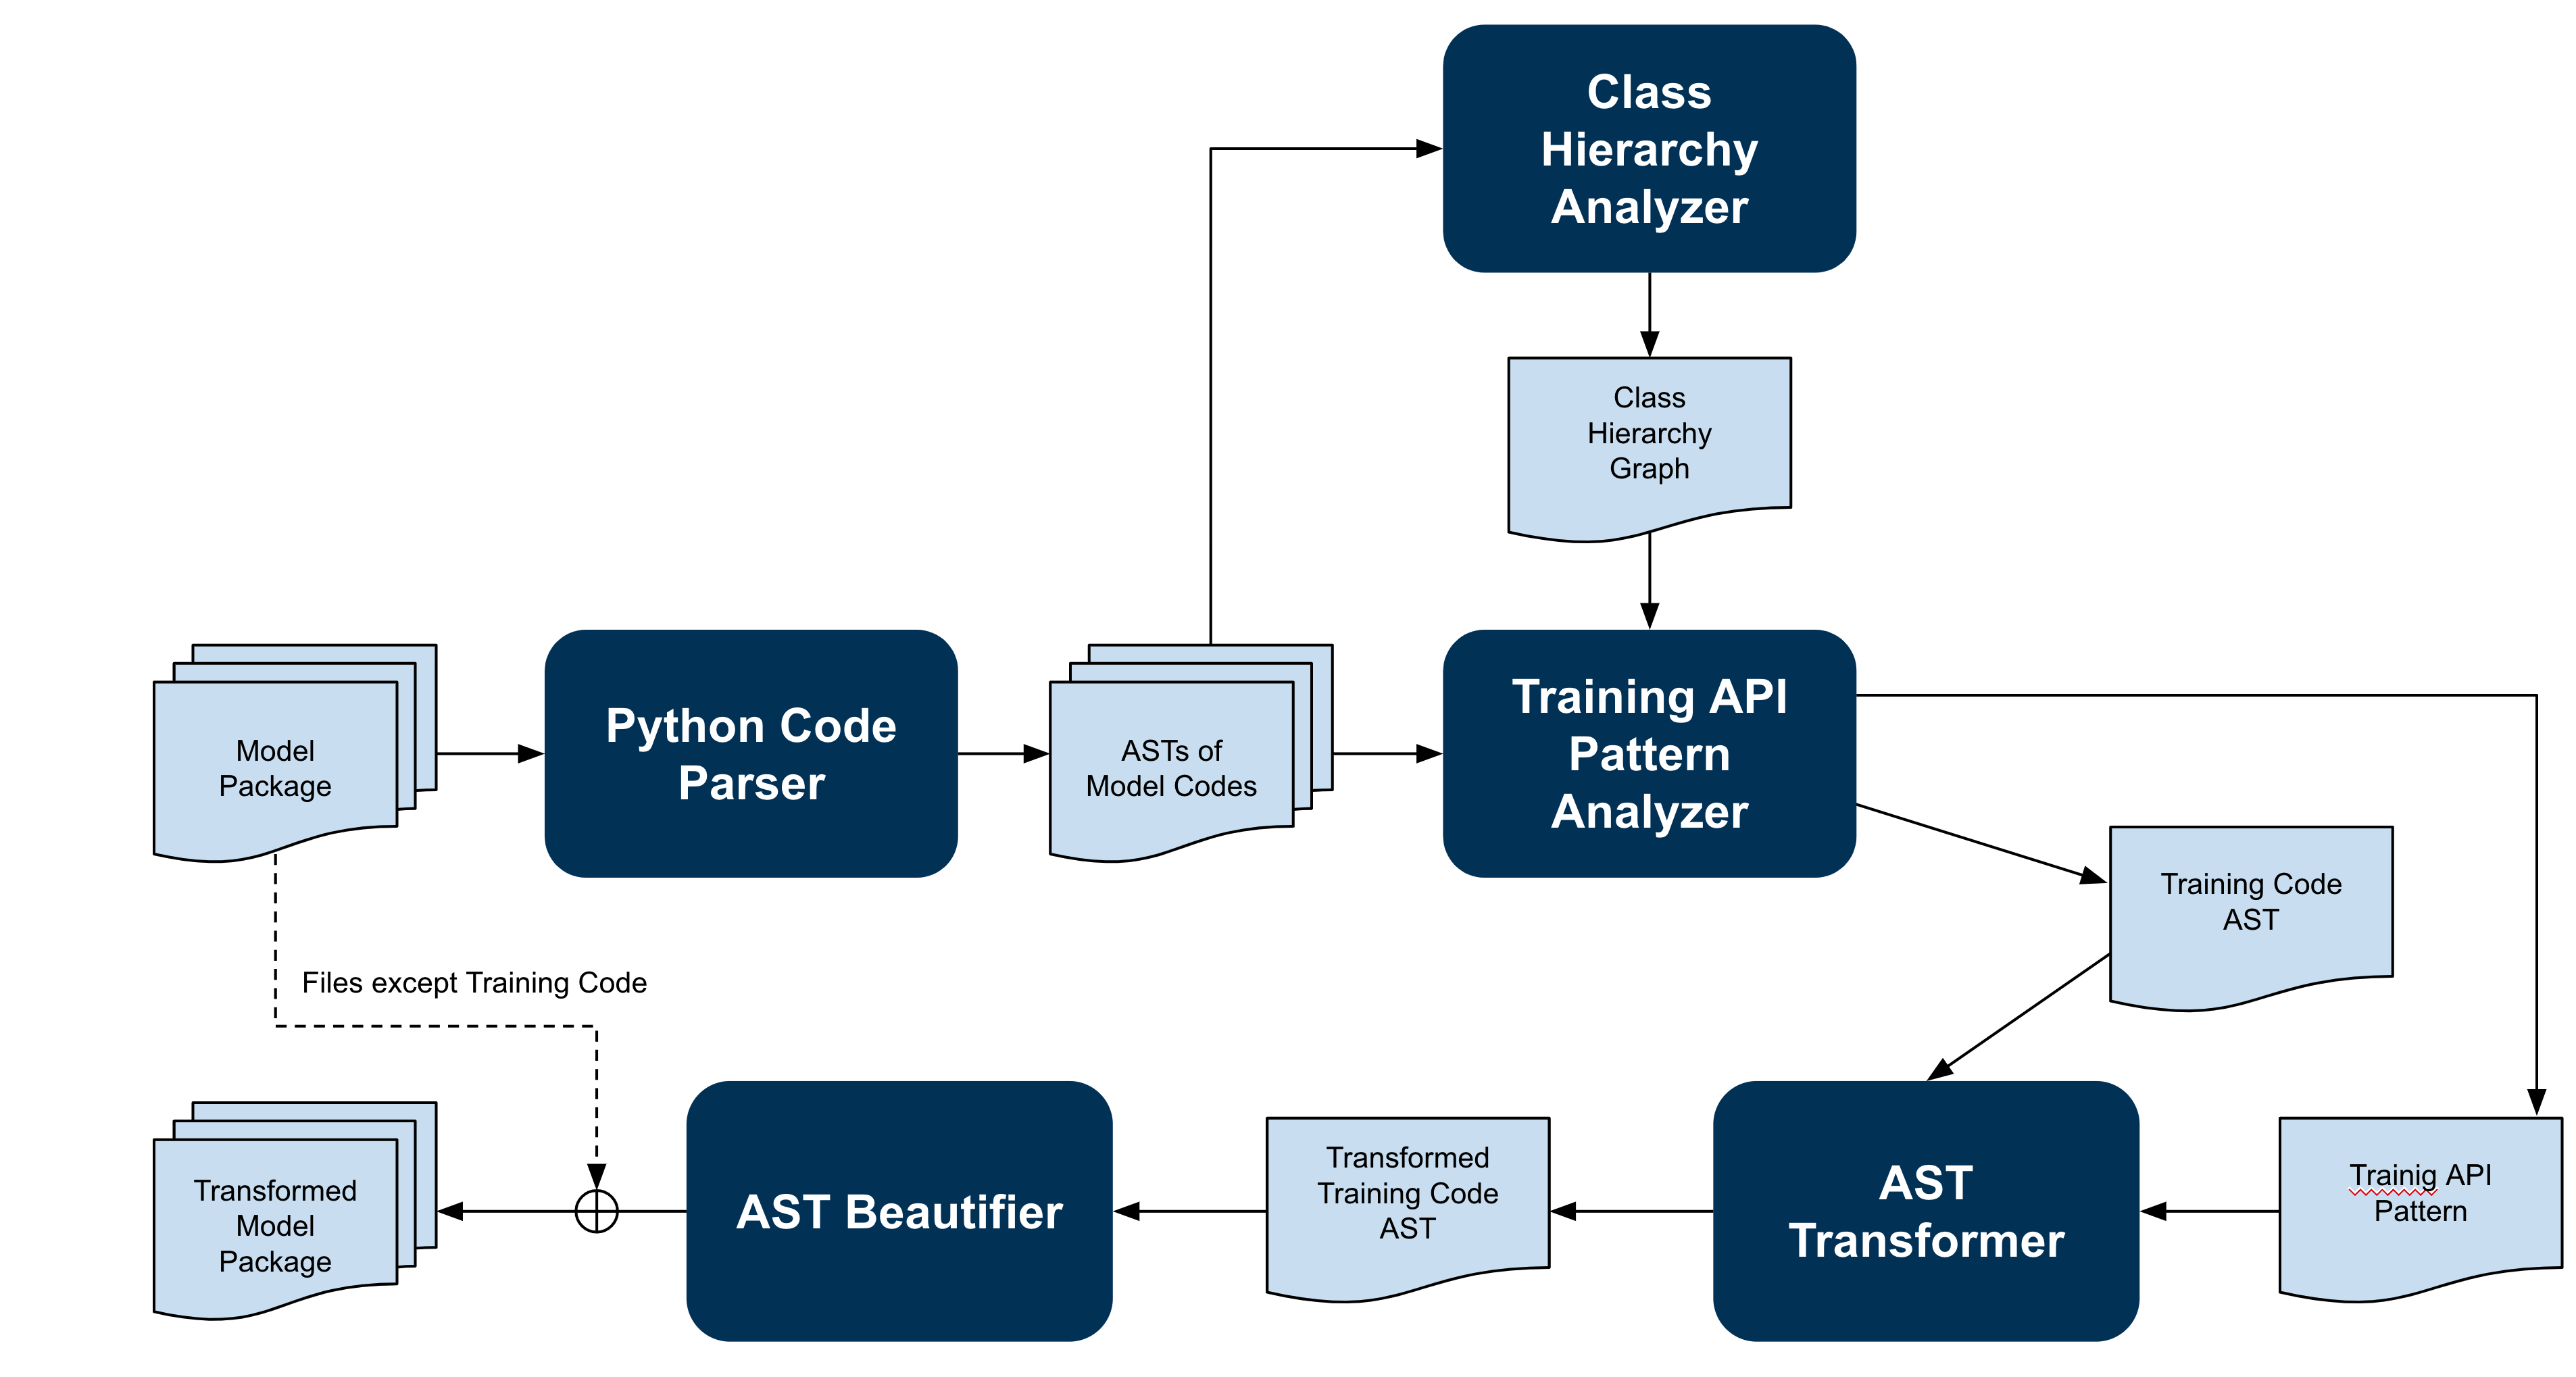
\includegraphics[width=15cm]{system_arch}

The figure illustrates the software architecture and workflow.
The software is composed of 5 modules:
Python code parser, class hierarchy analyzer,
training API pattern anlayzer, AST transformer, and AST beautifier.
The parser module parses Python codes in the input model package into 
a set of ASTs. Then the class hierarchy analyzer module 
produces a class hierarchy graph of the model package.
The training API pattern analyzer module receives the AST set and
the class hierarchy graph, identified the training code AST and
its tranining API pattern. The AST transformer module
transforms the tranining code AST according to the transformation rule.
The transformed traning code AST is printed as a Python code in the
AST beautifier module, to be merged with the original model package
and become the transformed model package.

\subsection{Class Hierarchy Analyzer}

The class hierarchy analyzer produces a class hierarchy graph, which
represents the subclassing relations between user-defined classes
and TensorFlow library classes that appear in the model code.
The class hierarchy graph is required by the training API pattern anlayzer;
thus, the class hierarchy analysis must occur before anlayzing the API pattern.

\lstinputlisting[language=Python]{subclass_ex.py}

The figure illustrates two Python codes, each defining a model structure
and training process. The ResNet model class is defined in `/model/ResNet.py',
which inherits the class `tf.keras.models.Model'.
This is a typical way to define a new ML model:
define a user-defined class that inherits a `tf.keras.models.Model'.
The training code `/train.py' then imports the model definition with
import statement in line 11.
The training proceeds by creating an instance of `ResNet' class
and calling the `fit' method.
In order to recognize that `/train.py' code is the training code,
the anlayzer must know that the `ResNet' class is indeed a model, that is,
a subclass of `tf.keras.models.Model'.
However, the anlayzer cannot infer that information
by only inspecting the `/train.py' code.
In order to infer that the `ResNet' is a subclass of the TensorFlow Model class,
class hierarchy information of the whole model package should first be generated.

There are several other TensorFlow classes that is inherited by user classes
to be used as an model training code component.
The class hierarchy analyzer module is responsible of identifying
such subclass relation over the model package and producing the
class hierarchy graph so that the training API pattern analyzer can
recognize the user-defined model components.

(TODO: impl detail)
In class hierarchy analysis, each class name is expressed as fully qualified name.
Here, fully qualified name of a class means qualified name\cite{???}
on the basis of top of the package.
That is, the path to the module where the class is defined
is used to express the fully qualified name of the class.
By using the fully qualified name, the same class name in different module
can be discriminated.

(how CHA work)

When class is declared, subclass relation is explicitly specified.
We collected all of this information in the class definition,
and we build a directed graph of subclass relation
where the node is fully qualified name and the directed edge exists
from the fully qualified name of child class to that of parent class.
Accordingly, to figure out whether some class X is subclass of some class Y,
we check whether there exists some path from the fully qualified name of X
to that of Y in the graph.

\subsection{Training API Pattern Analyzer}
Describe detailed explanation of TAPA.

(necessity of TAPA)

As mentioned in Section 2.1, user can choose which APIs to use
when building model using TensorFlow library.
However, different transformation rule should be applied
to different usage pattern of training API.
To apply appropriate rule to each model,
the training API pattern is analyzed before the transformation.

(categories of TAP)

First, we categorized the training API pattern into 4 categories:
Session/MonitoredSession, low-level API using TensorFlow1;
Estimator, high-level API using TensorFlow1;
DistributedGradientTape, low-level API using TensorFlow2;
and Keras, high-level API using TensorFlow2.
(TODO: show the category into a table)

(how TAPA work)

Each category has unique pattern of using training API.
For example, Keras pattern is 1) making instance of model and
2) call compile and fit method of that model.
Conversly, if call expressions of the method model.compile and model.fit are detected
where model is an instance of subclass of Model class in TensorFlow library,
we categorize it as Keras pattern.

(result of TAPA)

By using training API pattern analyzer, we can figure out the API pattern.
However, it is possible that model uses more than one categories of API pattern
such as using both low-level and high-level APIs.
In this case, we reject to transform because we assumes
that each model uses only one training API pattern in the transformation rule.

\subsection{AST Transformer}
Describe detailed explanation of AST Transformer.

In transformation, it takes results of class hierarchy analysis
and training API pattern analysis, and it transforms the code
according to the rule mentioned in Section 3.2.
Because of dynamic behaviors of Python, we give up soundness
to get more complete result.
We leaves warning log with some suggestions
when transformation rule is potentially inaccurate.

